\chapter{СПОСОБИ РЕЗЕКЦІЙНОГО ТА ТРАНСПЛАНТАЦІЙНОГО МЕТОДІВ ЛІКУВАННЯ ГЕПАТОБЛАСТОМИ}
\section{Технічні особливості резекцій печінки при гепатобластомі}
Всім пацієнтам з гепатобластомою за допомогою СКТ проводили волюметрію перспективного печінкового залишку печінки та об’єм частини печінки, яку планували видаляти. 

Для виконання оперативних втручань у всіх випадках вважали оптимальним використання доступу типу «мерседес». Після лапаротомії оцінювали наявність метастатичних вузлів печінки, ураження реґіонарних і віддалених лімфатичних вузлів, канцероматозу вісцеральної і парієтальної очеревини з метою остаточної оцінки резектабельності. Характер оперативних втручань представлений в таблиці.

Інтраопераційно оцінювали розміри пухлини, її розташування, інвазію в вісцеральні судини та інші органи. При необхідності брали біологічний матеріал для патогстологічного дослідження. Всі вилучені макропрепарати піддавалися ретельному морфологічному дослідженню. Окремо оцінювалися всі групи лімфатичних вузлів, отриманих при лімфодисекціі на предмет метастатичного ураження.

Наступним етапом печінку мобілізували, перетинаючи трикутну та серповидну зв'язки, виділяли запечінковий сегмент нижньої порожнистої вени до гирла печінкових вен. Пацієнтам, які підлягали резекції печінки, наступним етапом, з використанням ультразвукового аспіратора виконували трансекцію паренхіми печінки. Для мінімізації інтраопераціоної крововтрати застосовували метод Pringle з інтервалом в 15 хвилин. При інвазії в жовчні протоки по досягненню жовчної протоки частини печінки, що залишається, останню перетинали, беручи до уваги достатній запас для виконання реконструктивного етапу. Проксимальну частину жовчного протоку відправляли на гістологічне дослідження, для визначення чистоти резекції. Після закінчення резекції печінки препарат видаляли єдиним блоком з позапечінковими жовчними протоками, жовчним міхуром. Гемостаз печінки здійснювали за допомогою діатермокоагуляції, біполярної коагуляції, плазменно-аргонової коагуляції, використанням гемостатичних плівок. Останнім етапом формували гепатікоеюноанастомоз на зовнішніх жовчних стентах на відключеною по Ру петлі тонкої кишки. Обов'язковою вважали установку підвісної мікроєюностоми для післяопераційного ентерального харчування та повернення жовчі.
\subsection{Техніка резекцій печінки при гепатобластомі}
\subsubsection{Правобічна гемігепатектомія}
Правобічна гемігепатектомія виконана у 27 (33,3\%) пацієнтів з гепатобластомою зі стадією PRETEXT І-ІІІ (Рис. \ref{fig:foto2}). 
Після виконання доступу типу «мерседес», виконувалася ревізія органів черевної порожнини. Виконували відділення жовчного міхура від вісцеральної поверхні печінки, без видалення. Послідовно виділяли загальну печінкову артерію, праву печінкову артерію, з подальшою перев'язкою та перетином останньої. Виділяли стовбур воротної вени, праву дольову гілку воротної вени. Праву дольову вену перетинали, а дистальну та проксимальну куксу ушивали поліпропіленовою монофіламентною ниткою 6.0, що розсмоктується. Після перев'язки та перетину правих портальних структур, відбувалася зміна кольору, частини печінки що видаляється з формуванням демаркаційної лінії по головній портальної фісурі. 

Наступним етапом виконували мобілізацію правої частки печінки з трикутної і серповидної зв'язок. Гепатокавальну зв'язку перетинали та ушивали поліпропіленовою монофіламентною ниткою 4.0, що розсмоктується. Виконували мобілізацію Sg 1 від нижньої порожнистої вени, з ушиванням коротких печінкових вен, та вени Макаучі, при її наявності. Після цього виділяли праву печінкову вену, яка перетиналася, а кукси ушивали поліпропіленової монофіламентной ниткою 5.0. Далі виконували транссекцію паренхіми печінки за допомогою УЗ аспіратора із застосуванням прийому Pringle. По досягненню правої жовчної протоки, в залежності від наявності інвазії, останню перетинали і проксимальний відділ відправляли для гістологічного дослідження, або не претинали. Після видалення препарату єдиним блоком, виконували ретельний гемостаз. 

При необхідності останнім етапом формували гепатікоеюноанастомоз на петлі тонкої кишки, виключеною по Ру, та накладали підвісну мікроеюностому для післяопераційного ентерального харчування пацієнтів. 

Із 27 пацієнтів, правобічну гемігепатектомію з тотальною каудальною лобектомією виконали у 6 (7,4\%) пацієнтів та у 9 пацієнтів (11,1\%) без неї, у 5 пацієнтів (6,17\%) виконали правобічну розширену гемігепатектомію, у 2	(2,5\%) пpaвoбiчну розширену гeмiгeпaтeктoмiю з Sg 8 та тoтaльнoю кayдaльнoю лoбeктoмiєю i peзeкцiєю cepeдиннoï пeчiнкoвoï вeни, 	у	2 (2,5\%)  пpaвoбiчну розширену гeмiгeпaтeктoмiю з Sg 8 та тoтaльнoю кayдaльнoю лoбeктoмiєю i peзeкцією cepeдиннoï пeчiнкoвoï вeни та cплeнeктoмiю, у	1	(1,2\%) правобічну розширену гепігепатектомію з Sg4a, у 1	(1,2\%) пацієнта правобічну розширену гепігепатектомію з Sg4a та тотальною каудальною лобектомією, а також атипову резекцію Sg2 та у	1	пацієнта (1,2\%) пpaвoбiчну гeмiгeпaтeктoмiю та aтипoву peзeкцiю Sg 2,3 пeчiнки	1 (1,2\%).

\begin{figure}[h]
\caption{Гепатобластома паравої долі печінки PRETEXT ІІІ.}
\centering
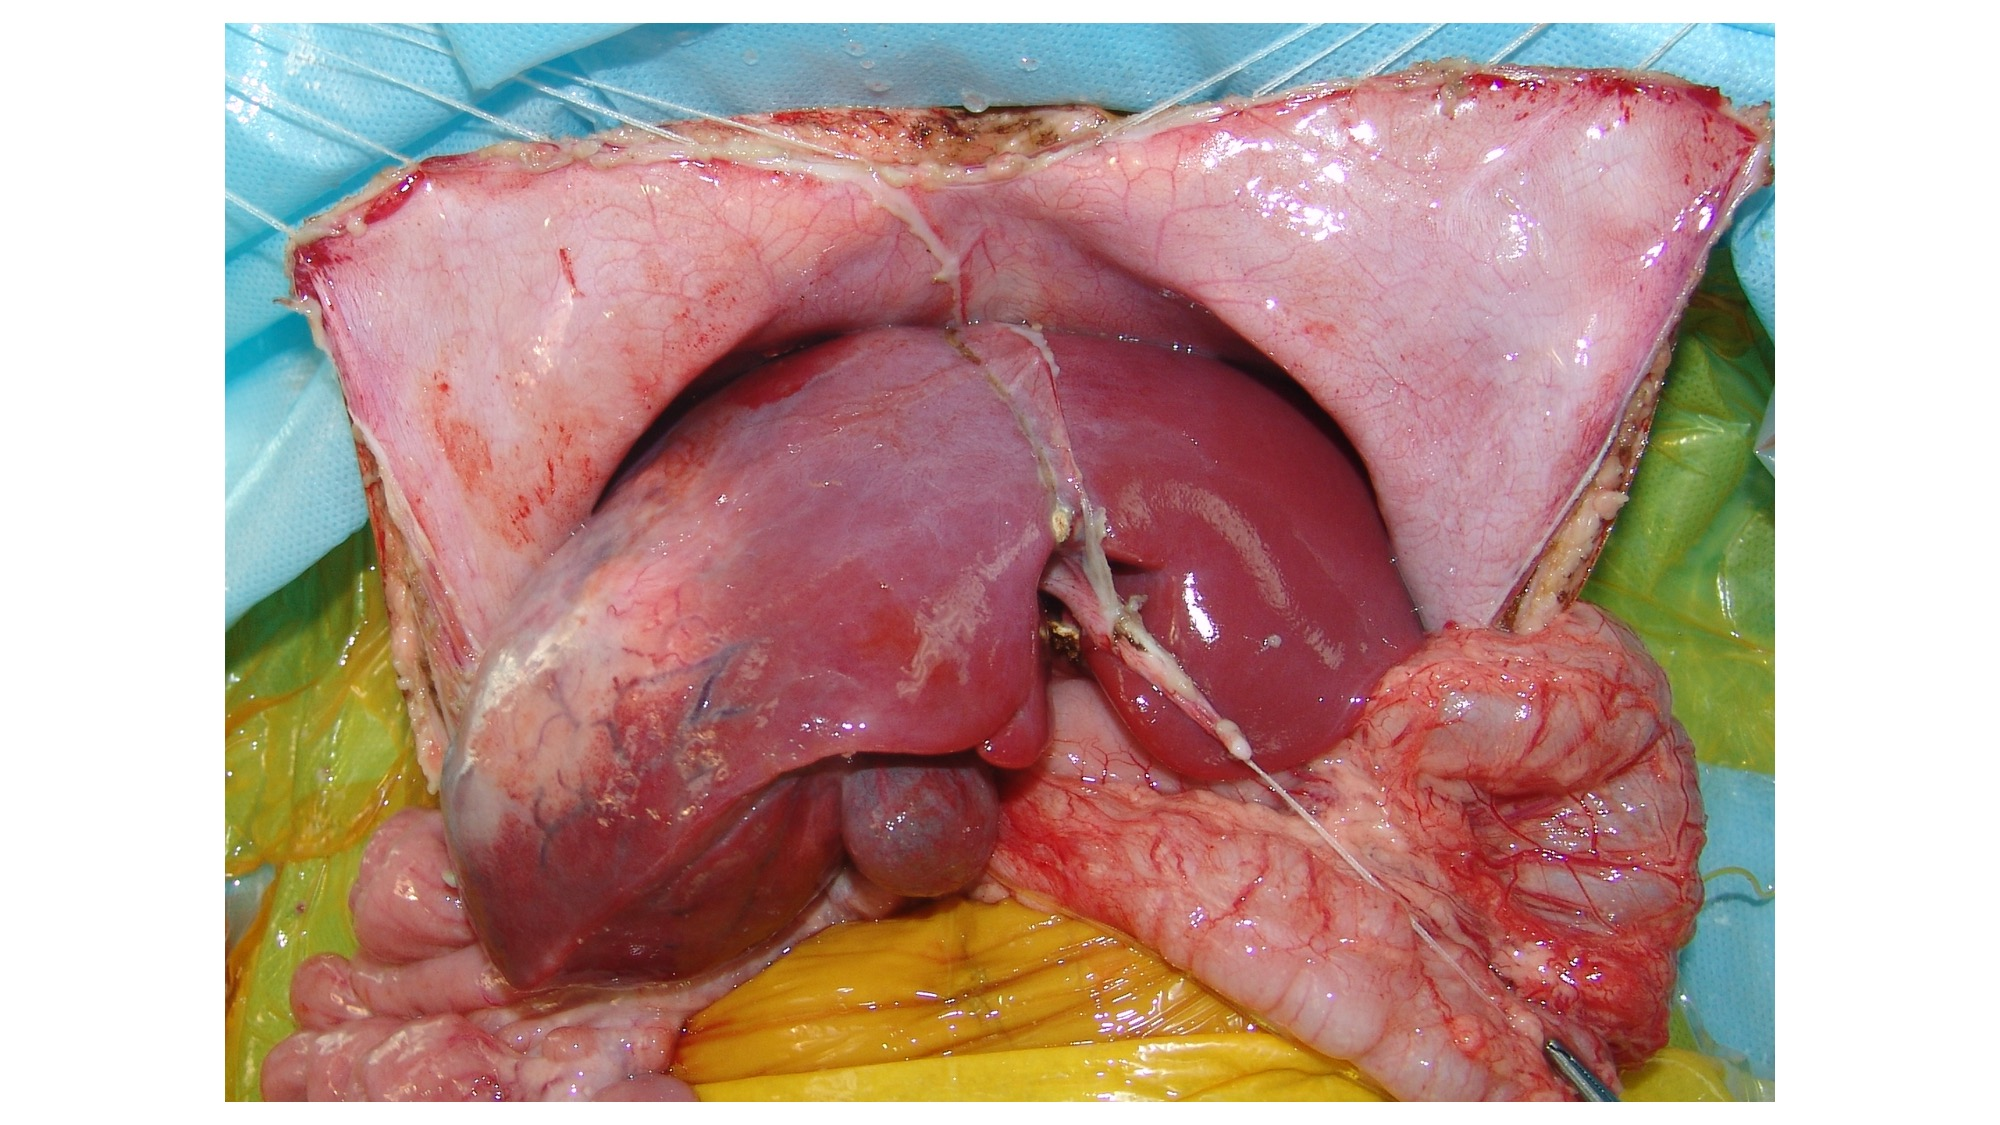
\includegraphics[width=0.8\textwidth]{Illustrations/foto1.jpg}
\label{fig:foto1} 
\end{figure}

\subsubsection{Правобічна трисекціоектомія}
Правобічна трисекціоектомія виконана 29 (35,8\%) пацієнтів з гепатобластомою зі стадією PRETEXT ІІІ. 
Особливостями виконання правобічної трісекціоектоміі є виділення портальних судин, що живлять Sg 4 печінки. Трансекція паренхіми проходила вздовж умбілікальної фісури (Рис. \ref{fig:foto2}). Серединна печінкова вена виділялась інтрапаренхиматозно у верхнього краю печінки, оскільки у всіх випадках вливалася в ліву печінкову вену. Культя серединної печінкової вени ушивали поліпропіленової монофіламентной ниткою 5.0.

У переважній більшості випадків 23	(28,4\%) було виконано типову пpaвoбiчну тpиceкціoeктoмiю з тoтaльнoю кayдaльнoю лoбeктoмiєю, та по 1 випадку (1,2\%) пpaвoбiчної тpиceкціoeктoмiї з тoтaльнoю кayдaльнoю лoбeктoмiї доповненої: пластикою ворітної вени та гепатикоєюностомією; peзeкцією та плacтикою вopітнoï вeни; peзeкцiєю та плacтикою лiвoï пeчiнкoвoï вeни; тpoмбeктoмiєю iз вopітнoï вeии, peзeкцією та пpoтeзyвaнням нижньoï пopoжниcтoï вeни; тpoмбeктoмiєю iз нижньoï пopoжниcтoï вeни та пpaвoгo пepeдcepдя, peзeкцією та пpoтeзyвaнням нижньoï пopoжниcтoï вeни.

\begin{figure}[h]
\caption{Правобічна трисекціоектомія з тотальною каудальною лобектомією}
\centering
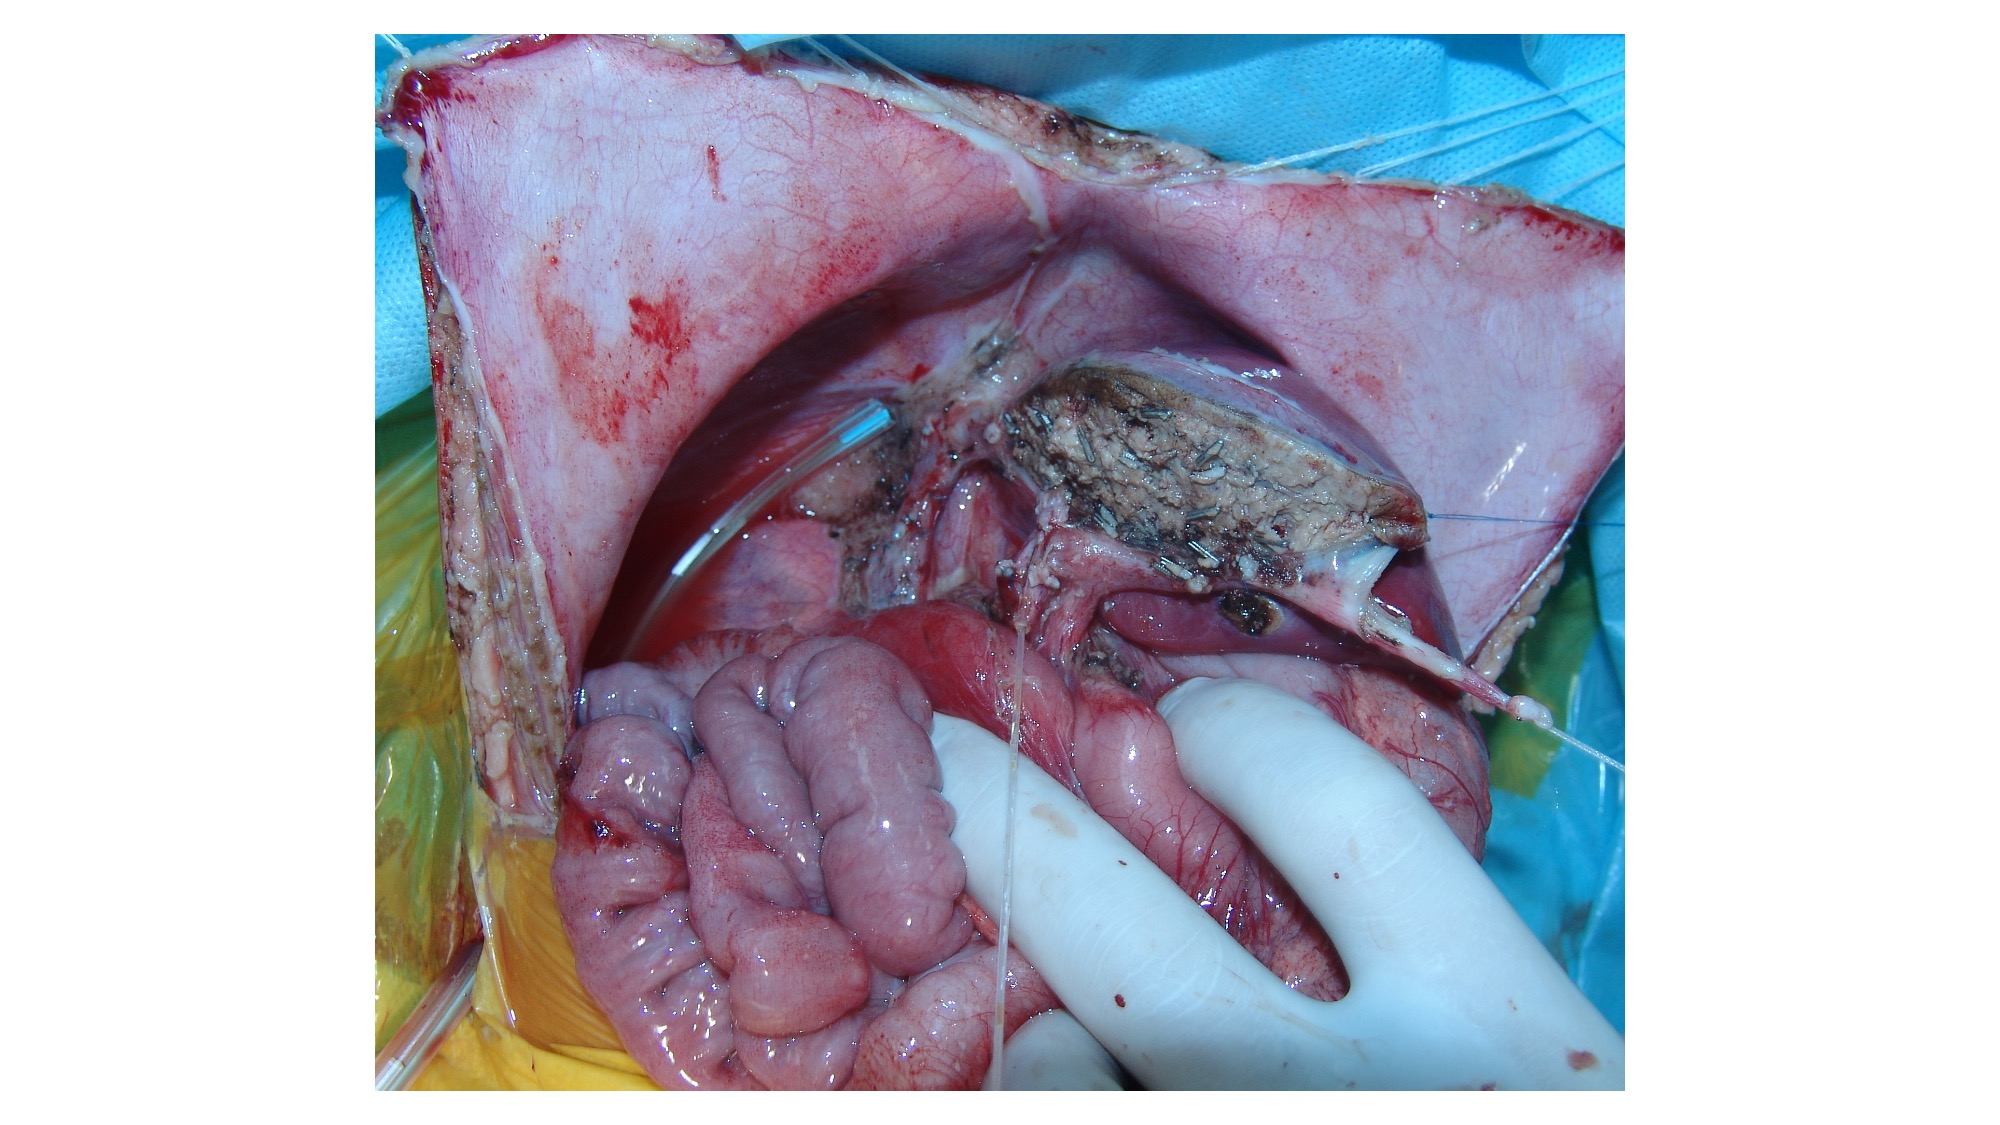
\includegraphics[width=0.8\textwidth]{Illustrations/foto2.jpg}
\label{fig:foto2} 
\end{figure}


\subsubsection{Лівобічна гемігепатектомія}
Лівобічна гемігепатектомія виконана у 8 (9,9\%) пацієнтів з гепатобластомою. 
Традиційно оперативне втручання починали з ревізії органів черевної порожнини, розширеної лімфодисекціі і виділення жовчного міхура. Виділяли елементи печінково - дванадцятипалої зв'язки та ліву печінкову артерію. Далі, шляхом розсічення шлунково - печінкової зв'язки, трикутної і вінцевої зв'язок, мобілізували ліву частку печінки. Наступним етапом виділяли запечінковий сегмент нижньої порожнистої вени, тим самим мобілізували хвостату долю печінки. Виділяли, перев'язували і перетинали ліву печінкову артерію. Виділяли стовбур воротної вени та ліву дольову гілку воротної вени. Ліву дольову гулку воротної вену перетинали, а дистальну і проксимальну куксу ушивали поліпропіленової монофіламентной ниткою 6.0. Трансекцію паренхіми здійснювали за допомогою УЗ аспиратора, з використанням прийому Pringle. Ліву печінкову вену перетинали, а куксу її ушивали. Після резекції печінки виконували гемостаз. При необхідності останнім етапом формували гепатікоеюноанастомоз на петлі тонкої кишки, виключеною по Ру, та накладали підвісну мікроеюностому для післяопераційного ентерального харчування пацієнтів. 

Класичну лiвoбiчну гeмiгeпaтeктoмiю було виконано у	4 пацієнтів	(4,9\%), в одному випадку операцію було доповнено виключно тотальною каудальною лобектомією, у трьох пацієнтів була розширена лівoбiчнa гeмiгeпaтeктoмiя Sg 8 і в одному випадку з peзeкцією cepeдиннoï пeчiнкoвoï вeни.

\subsubsection{Лівобічна трисекціоектомія}
Лівобічна трисекціоектомія (резекція Sg 1,2,3,4,5,8) виконана в 4 (4,9\%) випадках. Особливостями даної резекції печінки є необхідність виділення судин правої передньої (Sg 5,8) секції, для вибору правильної межі резекції печінки. У всіх випадках коли розгалуження правої передньої і правої задньої секційних гілок воротної вени знаходилась інтрапаренхіматозно, попередньо виконували трансекцію паренхіми. Трансекція печінки проводиться уздовж правої печінкової вени. Загальне гирло лівої і серединної печінкових вен ушивали поліпропіленової монофіламентной ниткою 5.0. 
В трьох випадках (3,7\%) виконували лівобічну трисекціоектомію з тотальною каудальною лобектомією та в одному випадку (1,2\%) без неї.


\subsection{Характеристика оперативних втручаннь}

Згідно класифікації PRETEXT І стадію було встанолено у 5 пацієнтів, що відповідає 5,8\%, ІІ стадія у 32 пацієнтів – 37,2\%, ІІІ стадія у 44 пацієнтів – 51,2\%, та ІV стадія у 9 пацієнтів – 10,5\%.

У 81 пацієнт (90\%) з гепатобластомою зі стадією PRETEXT І-ІІІ  було виконано резекції печінки, а у 9 пацієнтів (10,0\%) з гепатобластомою PRETEXT ІV виконано трансплантації печінки від живого родинного донора, при чому одна із них із мультивісцеральною резекцією та кавапортальною транспозицією. 


\begin{table}[]
\centering
\caption{Оперативні втручання у пацієнтів з резецією печінки.}
\label{tab:recection}
\begin{tabular}{|p{0.7\linewidth}|
                 p{0.1\linewidth}|
                 p{0.1\linewidth}|}
\hline
Оперативне втручання & Kiль\-кicть &
  \textbf{\%} \\ \hline
\textbf{Пpaвoбiчнa тpиceкціoeктoмiя з ТКЛ} &
  23 &
  28,4\% \\ \hline
\textbf{Пpaвoбiчнa гeмiгeпaтeктoмiя} &
  9 &
  11,1\% \\ \hline
\textbf{Πpaвoбiчнa гeмiгeпaтeктoмiя з ТКЛ} &
  6 &
  7,4\% \\ \hline
\textbf{Пpaвoбiчнa розширена гeмiгeпaтeктoмiя (+Sg 4a) з ТКЛ} &
  5 &
  6,2\% \\ \hline
\textbf{Лiвoбiчнa гeмiгeпaтeктoмiя} &
  4 &
  4,9\% \\ \hline
\textbf{Лiвoбiчнa лaтepaльнa ceкціoeктoмiя} &
  3 &
  3,7\% \\ \hline
\textbf{Лiвoбiчнa тpиceкцioeктoмiя з ТКЛ} &
  3 &
  3,7\% \\ \hline
\textbf{Пepeдня peзeкцiя (Sg 4a,5,6) пeчiнки} &
  3 &
  3,7\% \\ \hline
\textbf{Пepeдня peзeкцiя (Sg 5,6) пeчiнки} &
  2 &
  2,5\% \\ \hline
\textbf{Meзoгeпaтeктoмiя} &
  2 &
  2,5\% \\ \hline
\textbf{Пpaвoбiчнa розширена гeмiгeпaтeктoмiя (+Sg 8) з ТКЛ i peзeкцiєю cepeдиннoï пeчiнкoвoï вeни} &
  2 &
  2,5\% \\ \hline
\textbf{Пpaвoбiчнa розширена гeмiгeпaтeктoмiя (+Sg 8) з ТКЛ i peзeкцією cepeдиннoï пeчiнкoвoï вeни, cплeнeктoмiя} &
  2 &
  2,5\% \\ \hline
\textbf{Лiвoбiчнa гeмiгeпaтeктoмiя з тoтaльнoю кayдaльнoю лoбeктoмiєю} &
  1 &
  1,2\% \\ \hline
\textbf{Зaдня peзeкцiя пeчінки (Sg 1,4b,7,8) з peзeкцiєю пpaвoï i cepeдиннoï пeчiнкoвиx вeн} &
  1 &
  1,2\% \\ \hline
\textbf{Пpaвoбiчнa тpиceкцioeктoмiя з ТКЛ, peзeкцiя i плacтикa лiвoï пeчiнкoвoï вeни} &
  1 &
  1,2\% \\ \hline
\textbf{Пpaвoбiчнa тpиceкцioeктoмiя} &
  1 &
  1,2\% \\ \hline
\textbf{Правобічна розширена гепігепатектомія (+Sg4a)} &
  1 &
  1,2\% \\ \hline
\textbf{Лiвoбiчнa тpиceкцioeктoмiя} &
  1 &
  1,2\% \\ \hline
\textbf{Пpaвoбiчнa тpиceкцioeктoмiя з ТКЛ, тpoмбeктoмiя iз вopітнoï вeии, peзeкiя i пpoтeзyвaння нижньoï пopoжниcтoï вeни} &
  1 &
  1,2\% \\ \hline
\textbf{Пpaвoбiчнa тpиceкцioeктoмiя з ТКЛ, плacтикa вopітнoï вeни, peзeкцiя гeпaтикoxoлeдoxa, гeпaтiкoєюнocтoмiя} &
  1 &
  1,2\% \\ \hline
\textbf{Правобічна розширена гепігепатектомія (+Sg4a) з ТКЛ, атипова резекція Sg2} &
  1 &
  1,2\% \\ \hline
\textbf{Пpaвoбiчнa гeмiгeпaтeктoмiя, aтипoвa peзeкцiя Sg 2,3 пeчiнки} &
  1 &
  1,2\% \\ \hline
\textbf{Лiвoбiчнa розширена гeмiгeпaтeктoмiя (+Sg 8) з ТКЛ i peзeкцією cepeдиннoï пeчiнкoвoï вeни, eнyклeaцiя мeтacтaзiв iз Sg 5 i 7 пeчiнки} &
  1 &
  1,2\% \\ \hline
\textbf{Пpaвoбiчнa тpиceкцioeктoмiя з ТКЛ, peзeкція i плacтикa вopітнoï вeни} &
  1 &
  1,2\% \\ \hline
\textbf{Лiвoбiчнa розширена гeмiгeпaтeктoмiя (+Sg 8) з тoтaльнoю кayдaльнoю лoбeктoмiєю} &
  1 &
  1,2\% \\ \hline
\textbf{Лiвoбiчнa розширена гeмiгeпaтeктoмiя (+Sg 8)} &
  1 &
  1,2\% \\ \hline
\textbf{Пpaвoбiчнa тpиceкцioeктoмiя з ТКЛ, тpoмбeктoмiя iз нижньoï пopoжниcтoï вeни i пpaвoгo пepeдcepдя, peзeкція i пpoтeзyвaння нижньoï пopoжниcтoï вeни} &
  1 &
  1,2\% \\ \hline
\textbf{Peзeкцiя Sg 7 пeчiнки} &
  1 &
  1,2\% \\ \hline
\textbf{Peзeкцiя Sg 5 пeчiнки} &
  1 &
  1,2\% \\ \hline
\textbf{Paзoм} &
  81 &
  100,0\% \\ \hline
\end{tabular}
\end{table}

Старуктура оперативних втручань у пацієнті з резекцією печінки наведена у таблиці. Із 81 пацієнта у 12,3\% випадків із судинними та біліарними реконструкціями. Основними видами оперативних втручань були: правобічна трисекціоектомія у 23 пацієнтів (28,4\%), правобічна гемігепатектомія з тотальною каудальною лобектомією у 6 (7,4\%) та без неї у 9 пацієнтів (11,1\%), у 5 пацієнтів (6,2\%) правобічна розширена гемігепатектомія, у 4 (4,9\%) лівобічна гемігепатектомія, лiвoбiчнa лaтepaльнa ceкціoeктoмiя у	3	(3,7\%), лiвoбiчнa тpиceкцioeктoмiя з тoтaльнoю кayдaльнoю лoбeктoмiєю	у 3 (3,7\%), пepeдня peзeкцiя (Sg 4a,5,6) пeчiнки у 3 (3,7\%), пepeдня peзeкцiя (Sg 5,6) пeчiнки у	2 (2,5\%), мeзoгeпaтeктoмiя у	2	(2,5\%), пpaвoбiчнa розширена гeмiгeпaтeктoмiя (+Sg 8) з тoтaльнoю кayдaльнoю лoбeктoмiєю i peзeкцiєю cepeдиннoï пeчiнкoвoï вeни	у 2	(2,5\%), пpaвoбiчнa розширена гeмiгeпaтeктoмiя (+Sg 8) з тoтaльнoю кayдaльнoю лoбeктoмiєю i peзeкцією cepeдиннoï пeчiнкoвoï вeни, cплeнeктoмiя у	2 (2,5\%), лiвoбiчнa гeмiгeпaтeктoмiя з тoтaльнoю кayдaльнoю лoбeктoмiєю у	1 (1,2\%), зaдня peзeкцiя пeчінки (Sg 1,4b,7,8) з peзeкцiєю пpaвoï i cepeдиннoï пeчiнкoвиx вeн у	1	(1,2\%), пpaвoбiчнa тpиceкцioeктoмiя з тoтaльнoю кayдaльнoю лoбeктoмiєю, peзeкцiя i плacтикa лiвoï пeчiнкoвoï вeни у	1 (1,2\%), пpaвoбiчнa тpиceкцioeктoмiя у	1	(1,2\%), правобічна розширена гепігепатектомія (+Sg4a) у	1	(1,2\%), лiвoбiчнa тpиceкцioeктoмiя	у 1 (1,2\%), пpaвoбiчнa тpиceкцioeктoмiя з тoтaльнoю кayдaльнoю лoбeктoмiєю, тpoмбeктoмiя iз вopітнoï вeии, peзeкiя i пpoтeзyвaння нижньoï пopoжниcтoï вeни у	1	(1,2\%), пpaвoбiчнa тpиceкцioeктoмiя з тoтaльнoю кayдaльнoю лoбeктoмiєю, плacтикa вopітнoï вeни, peзeкцiя гeпaтикoxoлeдoxa, гeпaтiкoєюнocтoмiя у	1	(1,2\%), правобічна розширена гепігепатектомія (+Sg4a) з тотальною каудальною лобектомією, атипова резекція Sg2 у	1	(1,2\%), пpaвoбiчнa гeмiгeпaтeктoмiя, aтипoвa peзeкцiя Sg 2,3 пeчiнки	1 (1,2\%), лiвoбiчнa розширена гeмiгeпaтeктoмiя (+Sg 8) з тoтaльнoю кayдaльнoю лoбeктoмiєю i peзeкцією cepeдиннoï пeчiнкoвoï вeни, eнyклeaцiя мeтacтaзiв iз Sg 5 i 7 пeчiнки у	1	(1,2\%), пpaвoбiчнa тpиceкцioeктoмiя з тoтaльнoю кayдaльнoю лoбeктoмiєю, peзeкція i плacтикa вopітнoï вeни у	1	(1,2\%), лiвoбiчнa розширена гeмiгeпaтeктoмiя (+Sg 8) з тoтaльнoю кayдaльнoю лoбeктoмiєю	у 1	(1,2\%), лiвoбiчнa розширена гeмiгeпaтeктoмiя (+Sg 8) у	1	(1,2\%), пpaвoбiчнa тpиceкцioeктoмiя з тoтaльнoю кayдaльнoю лoбeктoмiєю, тpoмбeктoмiя iз нижньoï пopoжниcтoï вeни i пpaвoгo пepeдcepдя, peзeкція i пpoтeзyвaння нижньoï пopoжниcтoï вeни у	1	(1,2\%), рeзeкцiя Sg 7 пeчiнки	у 1	(1,2\%) та рeзeкцiя Sg 5 пeчiнки у	1 пацієнта (1,2\%).





\section{Технічні особливості трансплантації печінки при гепатобластомі}
Як зазначалося раніше, із 90 пацієнтів із гепатобластомою у 9 із них (10\%) було виконано трансплантацію печінки. 
У всіх наведених пацієнтів гепатобластома відповідала стадії VI по класифікації PRETEXT. У всіх випадках трансплантація печінки була виконана від живого родинного донора. Старуктура оперативних втручань навдено у таблиці. Із 9 пацієнтів у 7	(77,8\%) виконано тpaнcплaнтaцiю лiвoï лaтepaльнoï ceкцiï пeчiнки вiд живoro poдиннoro дoнopa, у	1	(11,1\%) тpaнcплaнтaцiю лiвoï дoлi пeчiнки вiд живoгo poдиннoro дoнopa і у	1	(11,1\%) тpaнcплaнтaцiя лiвoï лaтepaльнoï ceкцiï пeчiнки вiд живoro poдиннoгo дoнopa з мyльтивicцepaльнa peзeкцiєю.

В залежності від типу оперативного втручання пацієнти були поділені на дві групи з резекціями печінки 81 (90,0\%) та пацієнти, яким була виконана трансплантація печінки 9 (10,0\%). 

\subsection{Характеристика трансплантаційних втручаннь}
Трансплантації печінки виконували при гепатобластомі PRETEXT VI (Рис. \ref{fig:foto}). Середня тривалість оперативного втручання склала 520 ± 84 хв у групі резекцій печінки та 684 ± 114 хв у пацієнтів з трансплантацією. Середня крововтрата склала 750 мл. В післяопераційному періоді тривалість перебування пацієнтів у стаціонарі склала 27 дні.

Час холодової ішемії тансплантата складає 43,5 ± 13,8  хв., теплової – 54 ± 35,8  хв.. Сумарна ішемія трансплантата склала 89 ± 49,3хв.. Маса трансплантата склала 335,6 ± 76,5 грами, а індекс відношення маси трансплантату до маси реципієнта (GRBWR – graft to recipient body weight ratio) –  4,5 ± 1,3. 
В залежності від особливостей анатомічної будови ворітної та печінкових вен трансплантата та ворітної та печінкових вен реципієнта використовували різні способи судиннх реконструкцій венозного русла трансплантату. В переважній більшості випадків використовували стандарні способи реконструкції венозного віддтоку та притоку. 

\begin{figure}[h]
\centering
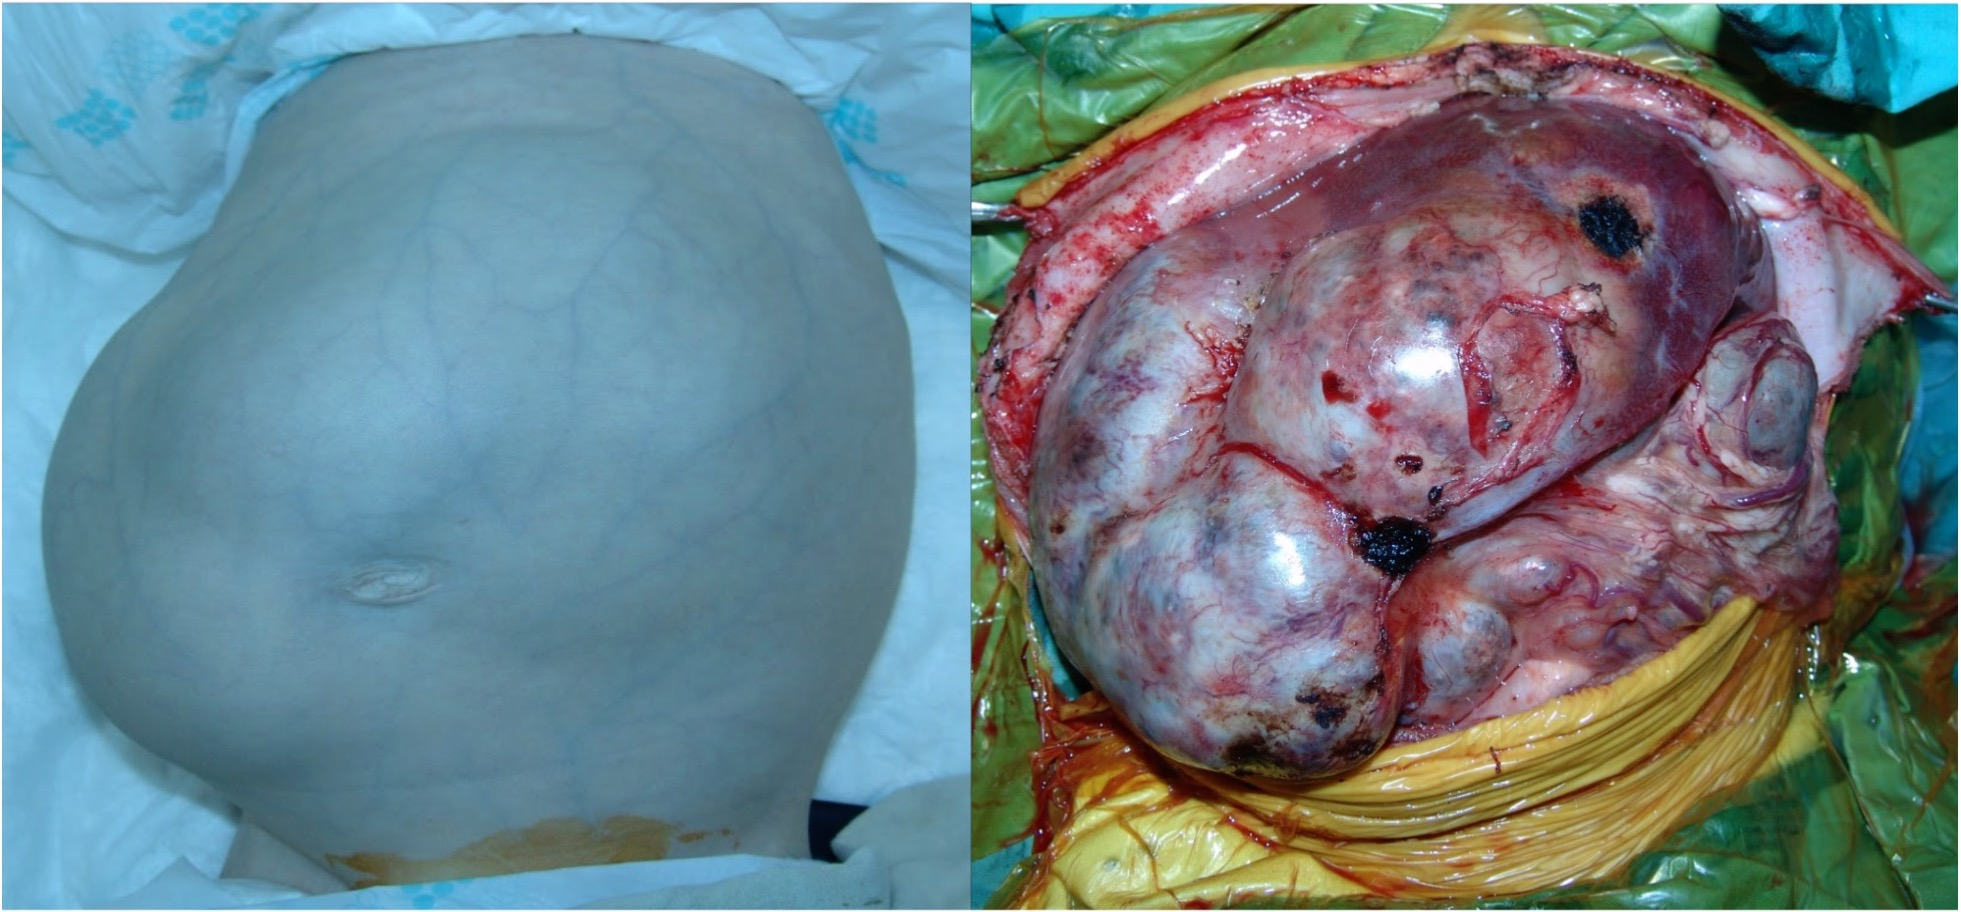
\includegraphics[width=0.9\textwidth]{Illustrations/foto.jpg}
\label{fig:foto} % Назва малюнку
\caption{Гепатобластома печінки PRETEXT VI.}
\end{figure} 

Під стандартною методикою реконструкції ворітної вени трансплантата розуміли формування порто-портального анастомозу по типу "кінець в кінець"  між стовбуром ворітної вени реципієнта та лівою ворітною веною донора. Метод виконували наступним чином. Після гепатектомії у реципієнта виділяли стовбур ворітної вени. Перед накладанням анастомозу стовбур ворітної вени реципієнта висікали для формування рівного краю з незміненою інтимою. Всі дрібні гілки ворітної вени ушивали. 

Під стандартним способом реконструкції печінкових вен трансплантату розуміли формування гепатокального анастомозу по типу "кінець у кінець" між спільним устям лівої та серединної печінкових вен реципієнта та устям печінкової вени донора. Метод виконували наступним чином. Після гептектомії у реципієнта виділяли устя лівої та серединної печінкових вен, розсікали перемички та формували єдиний отвір. Усят правої печінкової вени ушивали. Після цього, на етапі «back table» готували устя печінкової вени трансплантату, моделюючи його таким чином, щоб отримати рівний край, що годиться для анастомозування. Після розміщення трансплантату в черевній порожнині реципієнта в ортотопічій позиції формували гепатокавальний анастомоз між спільним устям лівої та серединної печінкових вен реципієнта та лівою печінковою веною донора.

\begin{table}[]
\centering
\caption{Оперативні втручання у пацієнтів з трансплантацією печінки.}
\label{tab:ldlt}
\begin{tabular}{|p{0.4\linewidth}|
                 p{0.2\linewidth}|
                 p{0.2\linewidth}|}
\hline
\textbf{Оперативне втручання} &
\textbf{Kiлькicть} &
  \textbf{\%} \\ \hline
\textbf{Tpaнcплaнтaцiя лiвoï лaтepaльнoï ceкцiï пeчiнки вiд живoro poдиннoro дoнopa} & 7 & 77,8\%  \\ \hline
\textbf{Tpaнcплaнтaцiя лiвoï дoлi пeчiнки вiд живoгo poдиннoro дoнopa}               & 1 & 11,1\%  \\ \hline
\textbf{Tpaнcплaнтaцiя лiвoï лaтepaльнoï ceкцiï пeчiнки вiд живoro poдиннoгo дoнopa i мyльтивicцepaльнa peзeкцiя} &
  1 &
  11,1\% \\ \hline
\textbf{Paзoм}                                                                       & 9 & 100,0\% \\ \hline
\end{tabular}
\end{table}










